\documentclass{article}
\usepackage{arxiv}

\usepackage[utf8]{inputenc} % allow utf-8 input
\usepackage[T1]{fontenc}    % use 8-bit T1 fonts
\usepackage{hyperref}       % hyperlinks
\usepackage{url}            % simple URL typesetting
\usepackage{amsfonts}       % blackboard math symbols
\usepackage{nicefrac}       % compact symbols for 1/2, etc.
\usepackage{microtype}      % microtypography
\usepackage{graphicx}

\usepackage{algorithm, algpseudocode}
\usepackage{amsmath}
\usepackage{bbold}
\usepackage{booktabs}
\usepackage{caption}
\usepackage{dirtree}
\usepackage{listings}
\usepackage{subcaption}

% Your project title
\title{Building Deep Neural Networks Robust Against Adversarial Attacks}

% Your name
\author{
  Anthony Dickson \\
  Department of Computer Science\\
  University of Otago\\
  \texttt{dican732@student.otago.ac.nz} \\
}

\begin{document}
\maketitle

\begin{abstract}
Deep neural networks, and in particular convolutional neural networks, have seen great success over recent years and have achieved state-of-the-art performance in a wide range of tasks. However, recent work has shown that these networks are vulnerable to adversarial attacks which cause these networks to fail spectacularly. In the case of image data perturbations as small as a single pixel have been shown to be enough to fool these networks into assigning incorrect labels with a high level of confidence, and even just small random translations and rotations can fool convolutional neural networks in a similar way.  A growing body of work has started on addressing these issues and offer ways of mitigating the effects of adversarial attacks. In this literature review I will give a brief overview of adversarial attacks and the methods proposed that aim to build neural networks robust against these attacks.
\end{abstract}

\begin{figure}[h!]
    \centering
    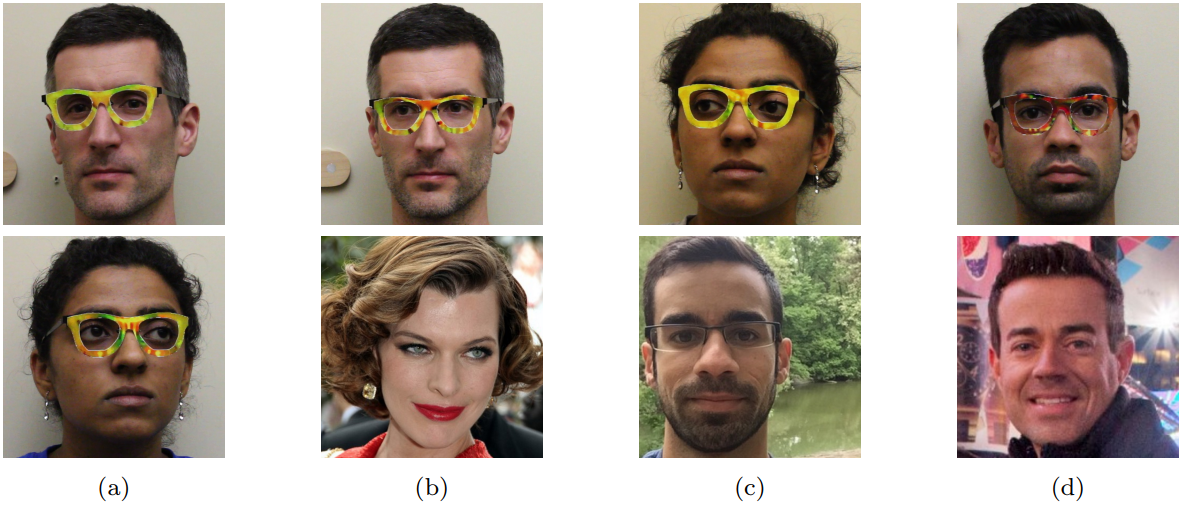
\includegraphics[width=\linewidth]{figures/dnn-impersonation.png}
    \caption{ Examples of successful impersonation attacks where a deep neural network (DNN) is forced to identify somebody as a specific person and dodging attacks where the DNN is forced to identify someone as anybody else. Figure (a) shows $S_A$ (subject A, top) and $S_B$ (subject B, bottom) dodging against a DNN. Figure (b)–(d) show impersonations. Impersonators carrying out the attack are shown in the top row and corresponding impersonation targets in the bottom row. Figure (b) shows $S_A$ impersonating Milla Jovovich (by Georges Biard; source: https://goo.gl/GlsWlC); (c) $S_B$ impersonating subject C $S_C$; and (d) $S_C$ impersonating Carson Daly (by Anthony Quintano; source: https://goo.gl/VfnDct).\protect\footnotemark}
    \label{fig:dnn_impersonation}
\end{figure}

\footnotetext{Figure and caption adapted from \cite{sharif2016accessorize}.}

\section{Introduction}
Convolutional neural networks have seen great success over recent years over a vast range of computer vision tasks \cite{lecun2010convolutional, krizhevsky2012imagenet, taigman2014deepface}. However, recent work has identified adversarial attacks that can cause state of the art deep neural networks (DNN) to fail spectacularly \cite{szegedy2013intriguing, goodfellow2014explaining, moosavi2016deepfool}. While most of the work on adversarial attacks has been focused on convolutional neural networks that deal with image data, there has been work showing that adversarial attacks are possible for other domains such as natural language processing and speech recognition \cite{papernot2016crafting, alzantot2018did}.

In the context of computer vision tasks, adversarial attacks perturb an image from the training dataset such that the target network assigns the incorrect label with a high level of confidence (see Figure \ref{fig:ostrich_examples}). The perturbations applied to the original images can be arbitrarily large or even as small as a single pixel \cite{su2019one}. Sometimes it is enough even to just randomly rotate and translate the image \cite{engstrom2017rotation}. These attacks are typically engineered such that the original image and adversarial example are indistinguishable to the human eye.

\begin{figure}
    \centering
    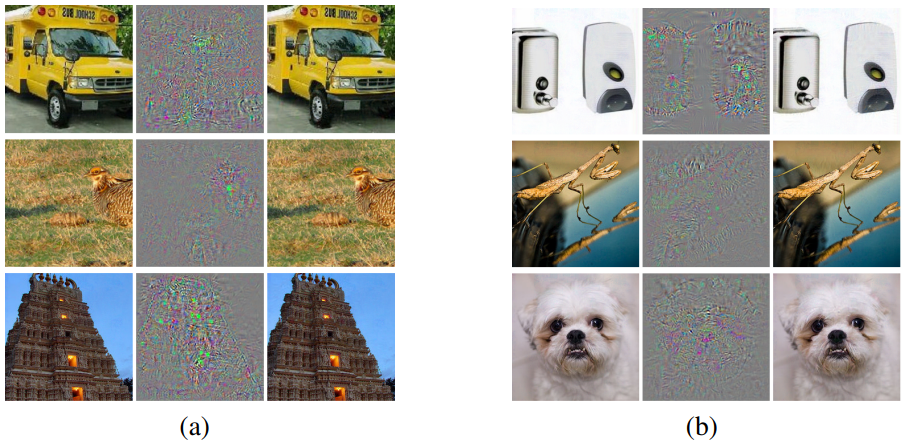
\includegraphics[width=\linewidth]{figures/adversarial-examples-ostrich.png}
    \caption{Adversarial examples generated for AlexNet \cite{krizhevsky2012imagenet}. (Left) is a correctly predicted sample, (center) difference between correct image, and image predicted incorrectly magnified by 10x (values shifted by 128 and clamped), (right) adversarial example. All images in the right column are predicted to be an \textit{``ostrich, Struthio camelus''}. Average distortion based on 64 examples is 0.006508. The examples are strictly randomly chosen. There is not any postselection involved.\protect\footnotemark}
    \label{fig:ostrich_examples}
\end{figure}

\footnotetext{Figure and caption adapted from \cite{szegedy2013intriguing}.}

There have been several theories proposed about how and why adversarial attacks work. Quoting the authors of \cite{schmidt2018adversarially}:  
\begin{quote}
Different works have argued that this vulnerability stems
from their discontinuous nature \cite{szegedy2013intriguing}, their linear nature \cite{goodfellow2014explaining}, or is a result of high-dimensional
geometry and independent of the model class \cite{gilmer2018adversarial}.
\end{quote}
An intriguing property of these adversarial attacks is that an adversarial example generated for a given network can successfully fool other networks, even ones that have a different architecture or were trained on different data \cite{szegedy2013intriguing}.

These vulnerabilities also raise questions about our understanding of the inner workings of convolutional neural networks. Previous work on visualising the features that convolutional neural networks (CNN) learn would suggest that these networks learn recognisable features \cite{simonyan2013deep, yosinski2015understanding, zintgraf2017visualizing}, and the fact that these networks create and use recognisable high-level features might suggest that these networks have a high-level understanding of visual data that is in some capacity comparable to that of humans.
However a recent study would suggest that CNNs are more sensitive to texture than to shape \cite{geirhos2018imagenet}, which is contrary to popular belief that CNNs recognise objects primarily through shape in a way similar to that of humans. 

Although machine learning agents built upon neural networks have been approaching human-level, or even super-human levels, of performance in various tasks \cite{taigman2014deepface, silver2017mastering}, it is concerning that they can be so easily fooled. The authors of \cite{sharif2016accessorize} highlight a particular concern regarding systems that use neural networks for facial recognition (see Figure \ref{fig:dnn_impersonation}), and how their vulnerability to adversarial attacks could possibly lead to security issues in such systems. 

This all goes to show that while CNN have reached impressive levels of performance, they are still far from being on par with humans in terms of robustness. So this leads me to the question:
\begin{quote}
    \textit{How can we can build neural networks that are robust against adversarial attacks?}
\end{quote} In this literature review I will provide a brief survey of some of the literature that addresses this question.

\section{Adversarial Training}
Szegedy et al. in their 2013 paper \cite{szegedy2013intriguing} were among the first to show the vulnerability of DNNs to adversarial examples. They formulate a method of constructing adversarial examples. They cast this problem as a box-constrained optimisation problem where they try to find a perturbation that results in a image that is as close as possible to the original image and causes the network to assign the wrong label. More formally they try solve the following optimisation problem:
\begin{center}
    Minimise $||r||_2$ subject to $f(x + r) = l$ and $x + r \in [0, 1]^m$
\end{center}
where $r$ is the perturbation to be applied to the input $x$, $f(.)$ is a function that maps an input to a label, $l$ is a label that differs from the correct label of $x$, and $m$ is the number of dimensions in the input. They use this method to generate adversarial examples for AlexNet and discover that these examples fool the network even though the examples are indistinguishable from the original images (see Figure \ref{fig:ostrich_examples}).

The authors then run a series of experiments to explore the effects of adversarial examples on generalisation. In their preliminary experiments they train a neural network with two hidden layers of 100 units each on the MNIST dataset and a pool of adversarial examples. The pool of adversarial examples are updated as training progresses. Their main result is that they were able to decrease the test error rate from 1.6\% to 1.2\% by training on adversarial examples. In other words, training the network on adversarial examples improved generalisation. 

In further experiments they explored how adversarial examples generated on one model \textit{generalise} to other models. They train five neural networks with either zero or two hidden layers and either 100 or 200 units in the hidden layers in a way similar to what was described above. Then they generated adversarial examples from each of these networks. They then fed these examples to the all of the other models other than the one that they were generated on. The interesting thing about their results is that sometimes the other networks were robust to the adversarial examples from the other networks only reporting an error rate of about 2.2\%. However, sometimes these networks would misclassify up to 87.1\% of these adversarial examples.

They further show that it is possible to train identical networks on subsets of the MNIST dataset, generate adversarial examples from the resulting networks, and fool the other networks with these examples. This method is slightly less effective, but nonetheless it demonstrates that adversarial examples are not particular to the network that generated them and generalise to some extent to other networks that either have a different architecture, were trained on a different set of data, or both.

They also run some informal experiments using convolutional neural networks. While they do not present the full results as with the fully connected neural networks trained on MNIST, the few examples they give are convincing (see Figure \ref{fig:ostrich_examples}) and serve as a motivating example for future work.

Overall Szegedy et al. bring forth the problem of adversarial attacks and propose a method for producing such examples. With their method they are able to consistently generate examples that fool a given network and are visually identical with the original image. They further show that these examples can fool networks that have a different architecture or networks with the same architecture that were trained on different sets of data. Their work does not necessarily give us any answers on how to build networks that is robust to adversarial attacks, but it does shows that incorporating adversarial examples into training data can improve generalisation on clean data. Their work also serves as the launching point for much of the work that has come afterwards.


\section{Robust Optimisation}
Rather than explicitly training on adversarial examples as Szegedy et al., later authors incorporate adversarial attacks into the optimisation process \cite{goodfellow2014explaining, madry2017towards, schmidt2018adversarially, yan2018deep}.

\subsection{Adversarial Loss as a Regulariser}
In \cite{goodfellow2014explaining} not only do Goodfellow et al. show that deep neural networks (DNN) can be fooled easily they also suggest several reasons as to why this happens. One of their main arguments is that DNNs are designed to be linear in order to facilitate efficient training, where they give examples such as the ReLU activation and manipulating activation values to be close to zero in sigmoid layers to avoid the effects of saturation (the sigmoid function near zero acts similar to a linear function).

They introduce a fast method for generating adversarial examples and explore how networks trained on MNIST cope with these. Their method, called the fast gradient sign method (FGSM), is defined as such:
\begin{equation} \label{eq:fgsm}
    \boldsymbol{\eta} = \epsilon \text{sign} (\nabla_{\mathbf{x}} J(\boldsymbol{\theta}, \mathbf{x}, y)).
\end{equation}
where $\boldsymbol{\eta}$ is the resulting perturbation, $\epsilon$ is some small scaling factor, $\boldsymbol{\theta}$ are the parameters of a model, $\mathbf{x}$ the input to the model, $y$ the targets/labels associated with $\mathbf{x}$, $J(\boldsymbol{\theta}, \mathbf{x}, y)$ is the loss to train the model with, and $\nabla_{\mathbf{x}} J(\boldsymbol{\theta}, \mathbf{x}, y)$ is the gradient of the loss function with respect to the input $\mathbf{x}$. 
Using FGSM they can construct an adversarial example by adding the perturbation $\boldsymbol{\eta}$ to the original input $x$. The reason why FGSM is fast is that once the gradient of the loss function with respect to the input is known an adversarial example can be made, whereas the method that Szegedy et al. introduced requires an iterative solution to be found via L-BFGS (an alternative optimisation algorithm to gradient descent) which can be slow.
While the quality of the solution found by the latter may be higher, FGSM is much faster and is still able to fool the networks consistently\footnote{They were able produce a set of adversarial examples that fooled the target with a 100\% success rate, whereas FGSM was only able to fool the target network 89.4\% of the time.}. An example of an adversarial example produced with FGSM is shown in Figure \ref{fig:panda_example_gibbon}.

\begin{figure}
    \centering
    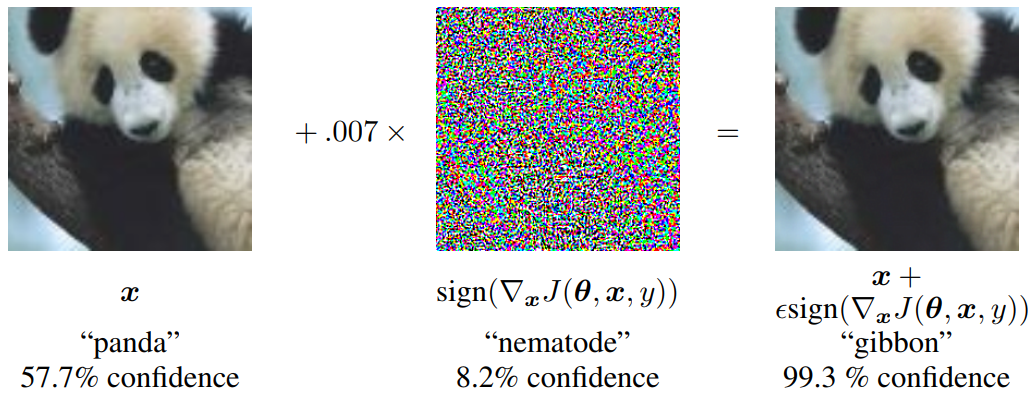
\includegraphics[width=\linewidth]{figures/panda-example-gibbon.png}
    \caption{A demonstration of fast adversarial example generation applied to GoogLeNet \cite{szegedy2015going} on ImageNet. By adding an imperceptibly small vector whose elements are equal to the sign of the elements of the gradient of the cost function with respect to the input, we can change GoogLeNet’s classification of the image. Here the $\epsilon$ of .007 corresponds to the magnitude of the smallest bit of an 8 bit image encoding after GoogLeNet’s conversion to real numbers.\protect\footnotemark}
    \label{fig:panda_example_gibbon}
\end{figure}
\footnotetext{Figure and caption adapted from \cite{goodfellow2014explaining}.}

They experiment with adversarial training on the MNIST dataset and with their method they are able to reduce the error rate of their neural networks from 89.4\% to about 17.9\% on a test set of adversarial examples.
They use a loss function that is a weighted sum of the loss on the clean input and the loss on the adversarial example:
\begin{equation*}
    \Tilde{J}(\boldsymbol{\theta}, \mathbf{x}, y) = \alpha J(\boldsymbol{\theta}, \mathbf{x}, y) + (1 - \alpha)J(\boldsymbol{\theta}, \mathbf{x} + \boldsymbol{\eta}).
\end{equation*}
where $\alpha$ is a scaling factor in the interval $[0, 1]$. In their experiments they set $\alpha=0.5$ which means they weighted the normal loss and the adversarial loss equally.
The second term acts sort of like a regularisation term.

Interestingly, while adversarially trained networks exhibit lower error rates, when they misclassified adversarial examples they still did so with a high level of confidence (on average about 81.4\%). So even with adversarial training there are still adversarial examples that fool the network with a high level of confidence. This suggests adversarial training does not make models that are impervious to further attacks. 
%The authors also experiment with radial basis function (RBF) networks, essentially neural networks with RBF activation functions (e.g. a Gaussian function). They found that this type of non-linear model is far less susceptible to adversarial attacks than typical neural networks, however they were . These two points would seem to support the argument that the linear models that are currently popular are inherently flawed. 
%Another interesting experiment that the authors do is train an ensemble of neural networks on different subsets of a data set and then measured the performance of the ensemble on adversarial examples, and even then the error rate was still high (~85-90\%).

\subsection{The Saddle-Point Problem}
In their 2017 work \cite{madry2017towards} Madry et al. take a slightly different view on the problem and investigate adversarial attacks under the lens of optimisation. They cast the problem of training robust models as a saddle-point problem for which if a good solution is found, then a guarantee can be made against the specific set of adversarial attacks that the saddle-point problem addresses.
The saddle-point problem they aim to solve is defined as such:
\begin{equation*}
    \displaystyle \min_{\theta} \rho(\theta) \text{ where } \rho(\theta) = \mathbb{E}_{(x, y) \sim D} \Big[\displaystyle \max_{\delta \in S} L(\theta, x + \delta, y)\Big]
\end{equation*}
where $\rho(.)$ is the outer loss function, $\theta$ is the model parameters, $\delta$ is perturbation from the set of allowed perturbations $S$, L(.) is the inner adversarial loss function, and $\mathbb{E}_{(x, y) \sim D} [\dots]$ is the expected value of the worst case adversarial attack for a given input $x$ and label $y$ that are part of the dataset $D$. The saddle-point problem also goes under the name of minimax in game theory, and we can indeed characterise this formulation as a model playing a sort of game against an adversary. In this imagined game the adversary is playing the role of saboteur and trying to fool the model with subtle modifications to the inputs and the model is trying to correctly label all of the inputs. 

They use FSGM (Equation \ref{eq:fgsm}) for generating adversarial examples. 
In their method they aim to train a robust DNN by first performing projected gradient descent (a bounded form of gradient descent) on the inner loss function to find the worst case adversarial attack, and then performing stochastic gradient descent to minimise the expected worst case adversarial loss. The authors remark that this is equivalent to performing SGD on adversarial examples (similar to what Szegedy et al. did in \cite{szegedy2013intriguing}), except that the main difference is that rather than training on a pool of pre-generated adversarial examples we are essentially creating a new adversarial example for each training example.
They argue that the above training method is not enough to create a robust model and that a higher model capacity is also required. Adversarial examples are said to create a more complex decision boundary. Thus a higher model capacity is needed to learn the more complex decision boundary in order for adversarial examples to be correctly classified. 
In further experiments the author show that using the strongest adversary and increased model capacity reduces the ability of adversarial examples to generalise between different models.

In \cite{schmidt2018adversarially} Schmidt et al. build upon previous work including work from \cite{madry2017towards}. They point out an interesting characteristic of DNNs trained on CIFAR10 compared to DNNs trained on MNIST: DNNs trained on adversarial examples for MNIST generalise well for both the original unperturbed examples and adversarial examples, however for DNNs trained on CIFAR10 there is a noticeable gap in generalisation between the original examples and adversarial examples. Their main argument is that many more examples are needed in order to produce robust classifiers. In their experiments they look at the effect of data set size on adversarial robustness. They show that for Gaussian distributed data (i.e. natural data) the class of model used does not matter (i.e. the adversarial vulnerabilities are more intrinsic to the data rather than the model) and linear models are able to achieve optimal robustness. Furthermore, they stated that ``robustness also strongly depends on properties of the underlying data distribution''. This statement leads nicely into the next paper that I will talk about.

\section{Adversarial Examples Are Not Bugs, They Are Features}
Most work to date has viewed adversarial examples as faults in the current systems, something that must be fixed. In recent paper Ilyas et al. take an interesting position on the topic \cite{ilyas2019adversarial}. Their position is that adversarial examples are a feature of the supervised learning paradigm.

In supervised learning the sole objective to minimise some loss function. Thus, a model is going to use any features available to it, even if the features are unintelligible to humans. These models have no inherent preference over which features it uses and they simply use whatever is a good predictor and leads to low loss. This means if we were to have two features, one that is a high-level feature such as a hand and another that is an ambiguous pattern of noise and assuming these features we equally predictive of the true label, then the model would use both.

This means that these models are going to rely on a combination of both robust and non-robust features. Ilyas et al. describe robust features as highly predictive features that are robust to adversarial perturbations and non-robust as features that are highly predictive but not robust against adversarial perturbations. If models rely on a combination of these robust and non-robust features then it follows that they will be vulnerable to adversarial attacks.

Their notion of robust and non-robust features also provide an explanation as to why adversarial examples generalise across models. They posit that these models are all learning similar non-robust features, and that the adversarial examples are taking advantage of these common features. They found that in popular machine learning datasets such as CIFAR10 and ImageNet that these robust and non-robust features are indeed present.

In one of their experiments they set out to provide some supporting evidence for the claim that the reliance on non-robust features is a cause of the vulnerability of DNNs to adversarial examples. They take the CIFAR10 dataset and produce two parallel datasets, one that contains solely robust features and another that contains solely non-robust features. An example is shown in Figure \ref{fig:robust_example}. As we can see in this example the non-robust feature looks quite similar to the adversarial perturbations. In their experiments both networks trained with the robust and non-robust datasets achieved roughly the same level of generalisation on the clean test set, however on the adversarial test set the network trained on the robust dataset achieved a higher level of accuracy. Perhaps as expected, the adversarially trained networks were more robust against adversarial examples.

\begin{figure}
    \centering
    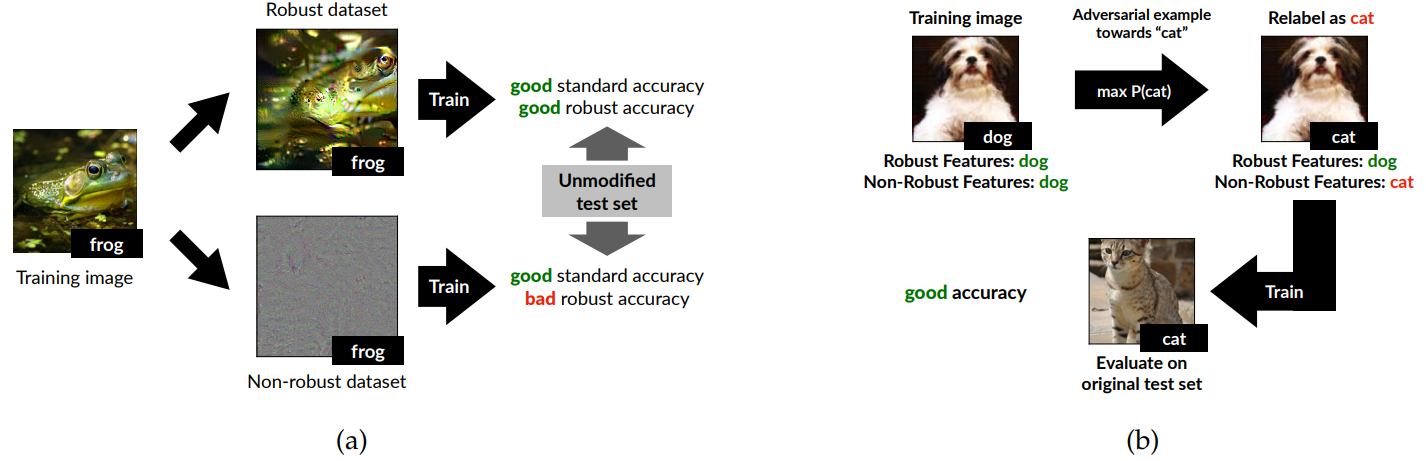
\includegraphics[width=\linewidth]{figures/robust-example.png}
    \caption{A conceptual diagram of the experiments performed in \cite{ilyas2019adversarial}. In (a) the authors disentangle features into combinations of robust/non-robust features (Section 3.1). In (b) the authors construct a dataset which appears mislabeled to humans (via adversarial examples) but results in good accuracy on the original test set.\protect\footnotemark}
    \label{fig:robust_example}
\end{figure}
\footnotetext{Figure and caption adapted from \cite{ilyas2019adversarial}.}

% One more work that deserves mention is Ilyas et al.'s 2019 paper \cite{ilyas2019adversarial}. They have an interesting perspective on the issue of the vulnerability of neural networks to adversarial attacks.
% Their main argument is that these vulnerabilities are the natural consequence of the supervised learning process and the features that the resulting model ends up relying on. In supervised learning the sole objective is to minimise the loss with respect to the model parameters (the weights and biases in the case of neural networks), and due that the models end up using any means available to them to do so. Furthermore, these models are no more likely to depend on higher level features such as ``ears'' than any other highly predictive pattern. They find that standard machine learning datasets such as CIFAR-10 contain highly predictive patterns that are unintelligible to humans and posit that DNNs end up relying on such patterns that lead to \textit{non-robust} features. Their main result is that by removing these highly predictive but imperceptible patterns they are able to train networks that are able to attain much higher accuracy on adversarial examples. Another interesting result is that there appears to be a trade-off between generalisation and the use of non-robust features, using more non-robust features seems to lead to better generalisation but the model ends up depending on more non-robust features and thus becomes more vulnerable to adversarial attacks.

% They conclude that:
% \begin{quote}
%     ``Our findings prompt us to view adversarial examples as a fundamentally \textit{human} phenomenon. In particular, we should not be surprised that classifiers exploit highly predictive features that happen to be
% non-robust under a human-selected notion of similarity, given such features exist in real-world datasets.
% In the same manner, from the perspective of interpretability, as long as models rely on these non-robust
% features, we cannot expect to have model explanations that are both human-meaningful and faithful to
% the models themselves. Overall, attaining models that are robust and interpretable will require explicitly
% encoding human priors into the training process.''
% \end{quote}

\subsection{An Interesting Link}
There is an interesting link between this paper and a paper \cite{geirhos2018imagenet} that is not directly related to adversarial attacks. In the latter they give evidence that suggests that DNNs trained on the ImageNet dataset are more sensitive to texture than to shape. That is to say that the networks they tested would make decisions/classifications based more on the texture of an image than the shapes present in it (see Figure \ref{fig:cat_shapes}). This runs in contrast to how humans are thought to be more focused on the shape of objects, rather than the texture. 

\begin{figure}
    \centering
    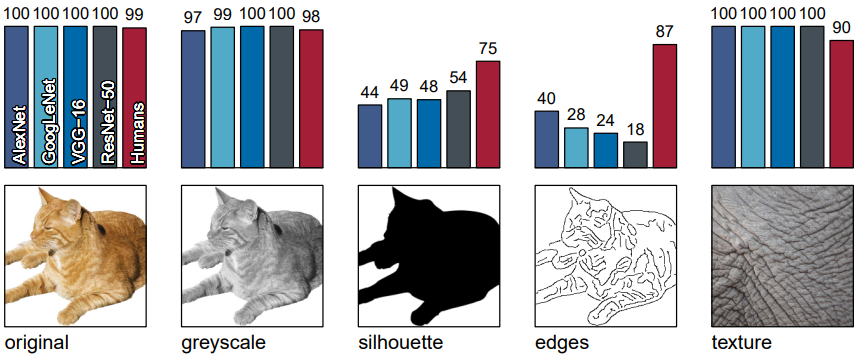
\includegraphics[width=\linewidth]{figures/cat-shape.png}
    \caption{Accuracy of predictions by various DNNs and human participants for varying stimuli. The first four images are of a cat and the last is of an Indian elephant's skin. Notice how on the first four images the human participants remained relatively confident that the image was of a cat, whereas the neural networks did not handle the silhouette or edges very well.\protect\footnotemark}
    \label{fig:cat_shapes}
\end{figure}
\footnotetext{Figure and caption adapted from \cite{geirhos2018imagenet}.}

The authors run experiments that make a DNN make decision based more on shapes than texture. They do this by using a technique called style transfer (see Figure \ref{fig:lemur_style_transfer}). The main idea behind this is that it severely weakens the correlation between texture and the class labels, thus forcing the networks to rely on other features instead of texture. An interesting result from their experiments is that forcing these networks to make decision based more on shape lead to them performing more closely to the human participants compared to the networks trained on just the original ImageNet dataset. 

So what is the link between this paper and Ilyas et al.'s work? It is possible that the reliance on texture by these models is in fact a reliance on non-robust features, and by decoupling texture from the labels the authors of \cite{geirhos2018imagenet} are actually forcing the networks to learn more robust features. Interestingly, in Ilyas et al.'s work there is a slight drop in generalisation of models trained solely on the robust features, and in Geirhos et al.'s work a similar thing happens when they train networks solely on the Stylized-ImageNet dataset. So it would appear that an interesting link exists between the two pieces work.


\begin{figure}
    \centering
    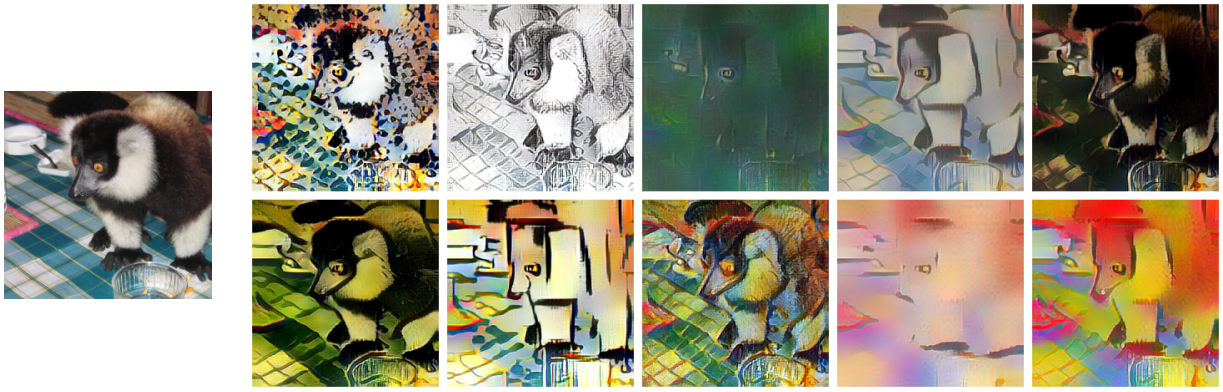
\includegraphics[width=\linewidth]{figures/lemur-style-transfer.png}
    \caption{Visualisation of Stylized-ImageNet (SIN), created by applying AdaIN style transfer to ImageNet images. Left: randomly selected ImageNet image of class ring-tailed lemur.
Right: ten examples of images with content/shape of left image and style/texture from different paintings. After applying AdaIN style transfer, local texture cues are no longer highly predictive of the target class, while the global shape tends to be retained. Note that within SIN, every source image is stylised only once.\protect\footnotemark}
    \label{fig:lemur_style_transfer}
\end{figure}
\footnotetext{Figure and caption adapted from \cite{geirhos2018imagenet}.}

\section{Discussion \&Conclusion}
Szegedy et al. brought attention to an intriguing property of neural networks (adversarial examples) in their 2013 work \cite{szegedy2013intriguing} which has prompted much research on the topic. They put forth a method for generating adversarial examples and showed that they generalise between different architectures and models trained on different sets of data. They also showed that training jointly on original data and adversarial examples can improve generalisation.

Following on from this paper there has been various attempts at explaining the vulnerability of neural networks to adversarial attacks and various methods for building neural networks that are robust to said attacks have been proposed. The main approach that I covered was the robust optimisation approach where adversarial attacks are built into the optimisation process. The authors of \cite{goodfellow2014explaining} propose a composite loss function that jointly considers the loss on the original input and the loss on the adversarial example. The authors of \cite{madry2017towards} and \cite{schmidt2018adversarially} cast the problem as solving the saddle-point problem where an inner function modelling adversarial loss is maximised, which essentially considers the worst case attack, and then minimises the loss with respect to this worst case attack. This approach builds robust networks that achieve high accuracy on adversarial examples.

Finally, the authors of \cite{ilyas2019adversarial} give an interesting perspective on adversarial attacks and suggest that they are a feature of the supervised learning process. They show that forcing the network to rely more on robust features results in networks that are more robust to adversarial examples, however the robust optimisation approach appears to be more effective. They also hint at a trade-off between generalisation ability and reliance on solely robust features. There is also an interesting link between this paper and \cite{geirhos2018imagenet} where the latter may provide an alternate high-level explanation as to why the standard training process leaves neural networks vulnerable to adversarial attacks.

One paper that I did not discuss is \cite{ye2018bayesian} which proposes giving neural networks the \textit{full Bayesian treatment} in order to make neural networks robust against adversarial attacks.

There is also an interesting similarity between robust optimisation methods for adversarial training and generative adversarial networks (GAN). Ian Goodfellow published the landmark paper on GANs in the same year that he published his other paper on adversarial attacks \cite{goodfellow2014explaining}. So I wonder if these methods were part of what inspired GANs. Furthermore, it would be interesting to see if the discriminator network part of GANs exhibit a similar level of adversarial robustness as networks trained with the robust optimisation methods.

\bibliographystyle{unsrt}
\bibliography{report}

\end{document}